% ============================================================
%  Mid-semester Project Review -- Beamer slides
%  Composing Context Compression for Long-Horizon LLM Agents
%  Theme: ufpel (theme .sty files + graphics/ must sit beside this file)
%  Compile with: pdflatex midreview_ppt.tex  (run twice)
% ============================================================
\documentclass[usenames,dvipsnames,aspectratio=169,10pt]{beamer}

\usetheme{ufpel}

\usepackage[T1]{fontenc}
\usepackage{lmodern}
\usepackage{amsmath,amssymb,mathtools}
\usepackage{booktabs}
\usepackage{graphicx}
\usepackage{tikz}
\usetikzlibrary{arrows.meta,positioning,calc,fit,shapes.geometric}
\usepackage{pgfplots}
\pgfplotsset{compat=1.16}

% title-page text sized for a long title
\setbeamerfont{title}{size=\LARGE,series=\bfseries}
\setbeamerfont{author}{size=\small}
\setbeamerfont{block title}{size=\normalsize}

% tighter lists
\setlength{\leftmargini}{1.4em}
\setlength{\leftmarginii}{1.2em}

% shorthand colours used across the diagrams
\definecolor{envblue}{RGB}{31,80,140}
\definecolor{cmpgreen}{RGB}{28,110,60}
\definecolor{ctlorange}{RGB}{190,105,10}
\definecolor{metviolet}{RGB}{110,45,140}

\title[Composing Context Compression for Long-Horizon LLM Agents]{Composing Context Compression\\for Long-Horizon LLM Agents}
\subtitle{Controlled Composition and Critical-Fact Retention on top of ACON}

\author[Ayush Rahate \& Rohit Chauhan]{%
  \textbf{123CS0006}~~Ayush Rahate \qquad \textbf{123CS0054}~~Rohit Chauhan\\[0.15cm]
  {\footnotesize \textbf{Project Supervisor:} Dr.~N.~Srinivas Naik}%
}

\institute[IIITDM Kurnool]{%
  {\small Department of Computer Science and Engineering\\
  Indian Institute of Information Technology\\
  Design and Manufacturing, Kurnool}%
}

\date[Mid-Sem Review]{\small Mid-Semester Project Review~~\textbar~~September 2026}

% ------------------------------------------------------------
\begin{document}

% ============================== 1. TITLE
\begin{frame}[plain]
  \titlepage
\end{frame}

% ============================== 3. MOTIVATION
\section{Motivation}

\begin{frame}{Context Grows Without Bound}
\begin{columns}[T]
\begin{column}{0.52\textwidth}
\centering
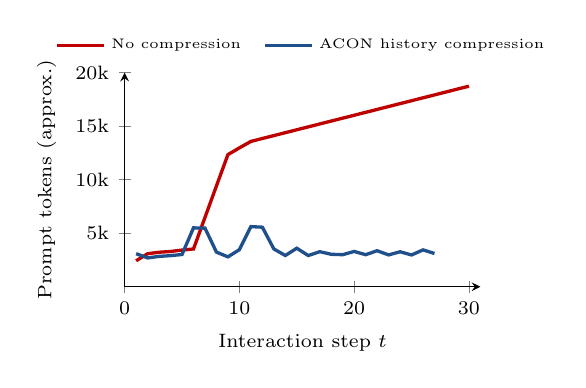
\begin{tikzpicture}[font=\scriptsize]
\begin{axis}[
  width=6.1cm, height=4.3cm,
  xlabel={Interaction step $t$},
  ylabel={Prompt tokens (approx.)},
  xmin=0, xmax=31, ymin=0, ymax=20000,
  ytick={5000,10000,15000,20000},
  yticklabels={5k,10k,15k,20k},
  scaled y ticks=false,
  xtick={0,10,20,30},
  axis lines=left,
  legend style={at={(0.5,1.04)},anchor=south,legend columns=2,draw=none,fill=none,
                font=\tiny,/tikz/every even column/.append style={column sep=6pt}},
]
\addplot[red!75!black, very thick] coordinates {
  (1,2425) (2,3085) (3,3223) (4,3292) (5,3427) (6,3527) (7,6472) (8,9424)
  (9,12348) (10,12974) (11,13580) (12,13851) (13,14123) (14,14394) (15,14666)
  (16,14937) (17,15209) (18,15480) (19,15752) (20,16023) (21,16295) (22,16566)
  (23,16838) (24,17109) (25,17381) (26,17652) (27,17924) (28,18195) (29,18467)
  (30,18738)};
\addlegendentry{No compression}
\addplot[envblue, very thick] coordinates {
  (1,3089) (2,2693) (3,2836) (4,2906) (5,3012) (6,5500) (7,5475) (8,3236)
  (9,2790) (10,3467) (11,5616) (12,5564) (13,3532) (14,2919) (15,3598)
  (16,2914) (17,3276) (18,3032) (19,2994) (20,3297) (21,2994) (22,3363)
  (23,2973) (24,3268) (25,2968) (26,3443) (27,3106)};
\addlegendentry{ACON history compression}
\end{axis}
\end{tikzpicture}

{\tiny \textbf{Our own runs}, AppWorld task \texttt{34d9492\_2} (both arms, 30
iterations). Baseline read from the agent's conversation log; the compressed
curve reconstructed from the 17 compressor-call records of the same task.
Tokens estimated at 4 characters/token. Peak: \textbf{18.7k} vs.\
\textbf{5.6k}.}
\end{column}
\begin{column}{0.46\textwidth}
\begin{alertblock}{Two bottlenecks}
\begin{itemize}\footnotesize
  \item \textbf{Memory} --- the KV cache scales with sequence length
  \item \textbf{Distraction} --- long, partly stale context degrades decisions
\end{itemize}
\end{alertblock}
\begin{block}{The tension}
\footnotesize
Compression must be \emph{aggressive} (to save tokens) and \emph{precise}
(one lost file path or API token derails an entire trajectory).
\end{block}
\end{column}
\end{columns}
\end{frame}

% ============================== BACKGROUND + LITERATURE
\section{Background and Related Work}

\begin{frame}{Methods We Build On, and the Field}
\begin{columns}[T]
\begin{column}{0.49\textwidth}
\begin{block}{ACON --- prompt-level, generative}
\scriptsize
\begin{itemize}
  \item An LLM \emph{rewrites} history when $|h_t|>T_{\mathrm{hist}}$, shortens
        observations when $|o_t|>T_{\mathrm{obs}}$
  \item Guideline optimised \emph{in natural language} by contrasting
        uncompressed successes with compressed failures
  \item Agent frozen; compressor distilled into a small model
  \item AppWorld: $56.5\%$ vs.\ $56.0\%$ acc., peak tokens $\downarrow$ 26--54\%
\end{itemize}
\end{block}
\end{column}
\begin{column}{0.49\textwidth}
\begin{block}{SAC --- KV-level, soft}
\scriptsize
\begin{itemize}
  \item Selects \emph{anchor tokens}, marks them with a learned embedding
  \item Bidirectional attention lets anchor KV absorb the whole context
  \item No autoencoding pretraining required
  \item MRQA, Llama-3.2-1B at $15\times$: $54.95$ ID F1 (EPL $51.52$)
\end{itemize}
\end{block}
\end{column}
\end{columns}

\vspace{0.15cm}
\centering
\tiny
\renewcommand{\arraystretch}{1.1}
\setlength{\tabcolsep}{3pt}
\resizebox{0.96\textwidth}{!}{%
\begin{tabular}{lcccccc}
\toprule
\textbf{Property} & \textbf{ACON} & \textbf{SAC} & \textbf{SWE-Pruner} &
\textbf{LLMLingua} & \textbf{MEM1/MemAgent} & \textbf{Proposed}\\
\midrule
Agent weights frozen     & Yes  & Yes & Yes & Yes & \textcolor{red!70!black}{No} & Yes\\
History compression      & Yes  & No  & No  & Yes & Merged & Yes\\
Observation compression  & Yes  & No  & Yes & Yes & Merged & Yes\\
Composition studied      & Partly & No & No & No & No & \textcolor{cmpgreen}{\textbf{Yes}}\\
Intrinsic quality metric & No   & No  & No  & No  & No & \textcolor{cmpgreen}{\textbf{Yes (CFR)}}\\
\bottomrule
\end{tabular}}

\vspace{0.15cm}
{\scriptsize Every existing method compresses \emph{one} kind of context ---
how the stages \textbf{interact} is unstudied.}
\end{frame}

% ============================== SETUP + ACON RESULTS
\section{Reproduction}

\begin{frame}{Result 1: ACON on AppWorld}
{\scriptsize
\textbf{Setup:} one RTX 2000 Ada (16\,GB), Ollama; agent \texttt{qwen2.5:14b},
compressor \texttt{qwen2.5:7b}; AppWorld \texttt{train\_history\_tiny}
(38 tasks), seed 42, temperature 0.}
\vspace{0.1cm}
\centering
\scriptsize
\renewcommand{\arraystretch}{1.15}
\setlength{\tabcolsep}{4.5pt}
\resizebox{\textwidth}{!}{%
\begin{tabular}{lcccccc}
\toprule
\textbf{Run} & \textbf{Tasks} & \textbf{Max iter.} & \textbf{Solved} &
\textbf{Avg iter.} & \textbf{Agent input tok.} & \textbf{Wall clock (s)}\\
\midrule
Baseline, no compression                          & 8  & 12 & 1 & 11.00 & 269,935 & 953.9\\
History compression ($T_{\mathrm{hist}}{=}512$)   & 8  & 12 & \textbf{2} & 10.75 & 232,749 & 882.8\\
Observation compression ($T_{\mathrm{obs}}{=}256$)& 8  & 12 & 1 & 11.00 & 261,422 & 873.6\\
\midrule
Baseline, full split                              & 38 & 30 & 12 (31.6\%) & 23.7 & 2,972,376 & 7312\\
\midrule
Baseline, matched subset                          & 18 & 30 & 7 & 22.22 & 1,283,906 & ---\\
History compression, matched subset               & 18 & 30 & \textbf{9} & 19.50 & \textbf{969,389} & ---\\
\bottomrule
\end{tabular}}

\vspace{0.2cm}
\begin{columns}[T]
\begin{column}{0.53\textwidth}
\scriptsize
\begin{itemize}
  \item 18 matched tasks: \textbf{9 solved vs.\ 7}, \textbf{24.5\% fewer}
        agent input tokens
  \item Not uniform: solved 5 the baseline failed, failed 3 it solved
  \item No latency overhead at this scale --- compressed runs finished sooner
\end{itemize}
\end{column}
\begin{column}{0.45\textwidth}
\begin{alertblock}{Caveats carried into every claim}
\scriptsize
Thresholds $512/256$ (paper: $4096/1024$, they rarely fire here);
4096-token serving window truncates long baseline prompts;
one seed per setting.
\end{alertblock}
\end{column}
\end{columns}
\end{frame}

% ============================== 8. SAC RESULTS
\begin{frame}{Result 2: SAC Reproduction and Pilot}
\begin{block}{SAC reproduces to within 0.2 F1}
\footnotesize
$15\times$: \textbf{54.98} ID / \textbf{39.25} OOD (published 54.95 / 39.26)
\qquad
$5\times$: \textbf{63.70} / \textbf{47.71} (published 63.63 / 47.72)
\end{block}
\vspace{-0.1cm}
\centering
\scriptsize
\renewcommand{\arraystretch}{1.2}
\setlength{\tabcolsep}{4.5pt}
\resizebox{\textwidth}{!}{%
\begin{tabular}{lcccc}
\toprule
\textbf{Run} & \textbf{ID F1} & \textbf{OOD F1} &
\textbf{$\Delta$ID vs.\ R0 (95\% CI)} & \textbf{$\Delta$OOD vs.\ R0 (95\% CI)}\\
\midrule
R0: SAC fine-tuning (matched control)  & 51.37 & 38.62 & control & control\\
R1: $+$ uniform KL (ablation)          & 51.06 & 38.17 & $-0.32\ [-1.02,+0.44]$ & $-0.45\ [-2.11,+1.44]$\\
R2: $+$ FGD (gated KL, $\lambda{=}1$)  & 51.15 & 38.47 & $-0.23\ [-0.95,+0.47]$ & $-0.14\ [-2.04,+1.77]$\\
R3: $+$ TGA $+$ FGD                    & \textbf{60.03} & \textbf{44.71} &
   $\mathbf{+8.66}\ [+7.66,+9.60]$ & $\mathbf{+6.10}\ [+3.62,+8.96]$\\
\midrule
\emph{Published SAC $15\times$ (20{,}000 steps)} & \emph{54.95} & \emph{39.26} & &\\
\bottomrule
\end{tabular}}



\vspace{0.3cm}
\begin{columns}
\begin{column}{0.92\textwidth}
\footnotesize
\begin{itemize}
  \item \textbf{FGD is a null result.} Its intervals contain zero. A diagnostic
        explains why: the zero-shot full-context teacher had \emph{higher}
        gold-answer NLL than the compressed student on \textbf{90.5\%} of
        2,000 training examples --- there is little to distil.
  \item \textbf{TGA\,$+$\,FGD wins}, beating the published 20,000-step
        checkpoint after a quarter of the budget --- but the question is seen
        during compression, so the memory is \emph{not reusable} across
        questions. This is a separate query-aware setting, not a drop-in
        improvement.
\end{itemize}
\end{column}
\end{columns}
\end{frame}

% ============================== RESEARCH GAPS (a)(b)(c)
\section{Research Gaps}

\begin{frame}{Three Gaps in Composition and Evaluation}
\begin{columns}[T]
\begin{column}{0.325\textwidth}
\begin{alertblock}{(a) Tokens $\neq$ time}
\scriptsize
The compressor is itself an autoregressive LLM call, and rewriting history
\textbf{invalidates the KV cache}, forcing the prefix to be re-encoded.
\vspace{0.1cm}

ACON's own medians (Qwen3-14B, one A100):
\vspace{0.05cm}

\centering
\begin{tabular}{lr}
No compression & 73.24\,s\\
History        & 87.68\,s\\
Observation    & 101.92\,s\\
\end{tabular}
\vspace{0.1cm}

\raggedright A token objective $C(\pi)$ misses this entirely.
\end{alertblock}
\end{column}
\begin{column}{0.335\textwidth}
\begin{alertblock}{(b) Schedule confound}
\scriptsize
The trigger set depends on the pipeline itself:
\vspace{-0.15cm}
\[
\mathcal{K}(\pi)=\big\{t : |h'_{t-1}\oplus(o'_t,a_t)|>T_{\mathrm{hist}}\big\}
\]
\vspace{-0.35cm}

Since $|o'_t|\le|o_t|$, compressing observations first shifts \emph{when}
history compression fires: $\mathcal{K}(\pi_{ho})\neq\mathcal{K}(\pi_h)$.
\vspace{-0.1cm}
\[
I=\Delta(\pi_{ho})-\Delta(\pi_h)-\Delta(\pi_o)=\mathbf{-9.5}
\]
\vspace{-0.4cm}

$I$ mixes composition with the shifted schedule, so it is \emph{not} evidence
that composition harms.
\end{alertblock}
\end{column}
\begin{column}{0.325\textwidth}
\begin{alertblock}{(c) Quality measured indirectly}
\scriptsize
ACON and SAC judge a compressor \textbf{solely} by downstream success:
\vspace{0.1cm}

\centering
$h'_t \;\rightarrow\;$ rollout $\;\rightarrow\; R$
\vspace{0.1cm}

\raggedright
A failure could mean the compressor dropped a needed fact, \emph{or} that the
agent reasoned badly. Neither method measures whether the facts the agent
\emph{will need} survive, so failures \textbf{cannot be attributed}.
\end{alertblock}
\end{column}
\end{columns}
\end{frame}

% ============================== 12. PROBLEM STATEMENT
\section{Problem Statement}

\begin{frame}{Problem Statement}
\begin{block}{Informally}
\scriptsize
Given a long-horizon agent with \textbf{frozen weights}, a history compressor
and an observation compressor, determine how the two stages should be
\textbf{composed and scheduled} so that the token savings of each are retained
without lowering task success --- holding the compression schedule fixed, and
measuring compression quality \emph{directly}.
\end{block}

\vspace{0.15cm}
{\scriptsize
\setlength{\abovedisplayskip}{4pt}\setlength{\belowdisplayskip}{6pt}
\setlength{\abovedisplayshortskip}{2pt}\setlength{\belowdisplayshortskip}{4pt}
\begin{columns}[T]
\begin{column}{0.49\textwidth}
\textbf{Agent (POMDP, frozen $\theta$):}
\[ a_t = M\big(h'_{t-1},\,o'_t;\,\theta\big) \]

\textbf{Compression operators:}
\[
o'_t=\begin{cases} f_o(o_t,h'_{t-1}) & |o_t|>T_{\mathrm{obs}}\\[2pt] o_t & \text{else}\end{cases}
\]
\[
h'_t=\begin{cases} f_h(x_t) & t\in\mathcal{K}\\[2pt] h'_{t-1}\oplus(o'_t,a_t) & \text{else}\end{cases}
\]

\textbf{Two composition orders} (ACON uses $x^{\mathrm{seq}}$)\textbf{:}
\[
\begin{aligned}
x_t^{\mathrm{seq}} &= h'_s\oplus(o'_{s+1},a_{s+1},\dots,o'_t,a_t)\\[2pt]
x_t^{\mathrm{dec}} &= h'_s\oplus(o_{s+1},a_{s+1},\dots,o_t,a_t)
\end{aligned}
\]
\end{column}
\begin{column}{0.49\textwidth}
\textbf{Cost, peak context and latency:}
\[ C(\pi)=\textstyle\sum_{t=1}^{T}\big(|h'_{t-1}|+|o'_t|\big) \]
\[ L(\pi)=\textstyle\sum_{t}\ell_M+\sum_{t\in\mathcal{K}}\ell_{f_h}
        +\sum_{|o_t|>T_{\mathrm{obs}}}\ell_{f_o} \]

\vspace{0.1cm}
\textbf{Formal objective:}
\[
\pi^{*}=\arg\max_{x,\;\mathcal{K}}\;
\mathbb{E}[R(\pi)]-\lambda\,\mathbb{E}[C(\pi)]-\mu\,\mathbb{E}[L(\pi)]
\]
\centering subject to
\[
\begin{aligned}
&\mathbb{E}[R(\pi)]\ge\mathbb{E}[R(\pi_\varnothing)]-\varepsilon\\[2pt]
&C(\pi_{ho})\le\min\{C(\pi_h),C(\pi_o)\}\\[2pt]
&\textcolor{cmpgreen}{\mathcal{K}(\pi_{ho})=\mathcal{K}(\pi_h)}
  \ \text{\tiny when comparing them}
\end{aligned}
\]
\end{column}
\end{columns}}
\end{frame}

% ============================== 13. PROPOSED PIPELINE
\section{Proposed Solution}

\begin{frame}{Proposed Pipeline}
\begin{center}
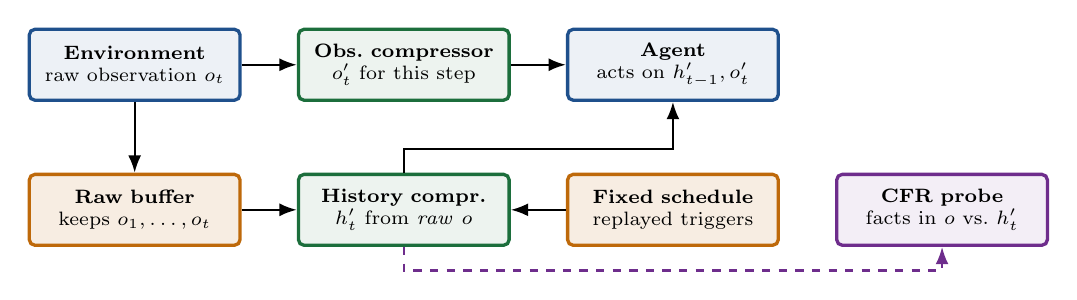
\begin{tikzpicture}[
  font=\scriptsize,
  bx/.style={draw, rounded corners=2pt, very thick, align=center,
    text width=2.5cm, minimum height=0.9cm, inner sep=2.5pt},
  arr/.style={-{Latex[length=2.2mm]}, line width=0.8pt},
  env/.style={bx, fill=envblue!8,  draw=envblue},
  cmp/.style={bx, fill=cmpgreen!8, draw=cmpgreen},
  ctl/.style={bx, fill=ctlorange!12, draw=ctlorange},
  met/.style={bx, fill=metviolet!8, draw=metviolet}
]
\node[env] (o) {\textbf{Environment}\\raw observation $o_t$};
\node[cmp, right=7mm of o]  (oc) {\textbf{Obs.\ compressor}\\$o'_t$ for this step};
\node[env, right=7mm of oc] (ag) {\textbf{Agent}\\acts on $h'_{t-1},o'_t$};
\node[ctl, below=9mm of o]  (buf){\textbf{Raw buffer}\\keeps $o_1,\dots,o_t$};
\node[cmp, right=7mm of buf](hc) {\textbf{History compr.}\\$h'_t$ from \emph{raw} $o$};
\node[ctl, right=7mm of hc] (sch){\textbf{Fixed schedule}\\replayed triggers};
\node[met, right=7mm of sch](cfr){\textbf{CFR probe}\\facts in $o$ vs.\ $h'_t$};
\draw[arr] (o)--(oc);
\draw[arr] (oc)--(ag);
\draw[arr] (o)--(buf);
\draw[arr] (buf)--(hc);
\draw[arr] (sch)--(hc);
\draw[arr] (hc.north) -- ++(0,0.3) -| (ag.south);
\draw[arr, dashed, metviolet] (hc.south) -- ++(0,-0.3) -| (cfr.south);
\end{tikzpicture}
\end{center}
\vspace{0.15cm}
\begin{columns}[T]
\begin{column}{0.49\textwidth}
\begin{block}{1. Decoupled composition order}
\footnotesize
The agent still gets the short $o'_t$, but the \textbf{raw} $o_t$ is kept in a
side buffer and $f_h$ receives $x^{\mathrm{dec}}_t$.
If $f_o$ only deletes content then $V(o'_t)\subseteq V(o_t)$, so facts dropped
by the observation stage \emph{can still reach} the history summary.
\end{block}
\end{column}
\begin{column}{0.49\textwidth}
\begin{block}{2. Controlled compression schedule}
\footnotesize
Record $\mathcal{K}^{h}=\mathcal{K}(\pi_h)$ from the history-only run and
\textbf{replay} it: $\mathcal{K}(\pi_{ho}):=\mathcal{K}^{h}$.
With the schedule fixed, $\pi_h$ and $\pi_{ho}$ differ \emph{only} in $f_o$,
so $I$ now measures composition alone.
\end{block}
\end{column}
\end{columns}
\end{frame}

% ============================== 14. CFR
\begin{frame}{Critical-Fact Retention (CFR)}
\begin{block}{Definition}
\footnotesize
Let $V(\cdot)$ extract state variables --- access tokens, entity IDs, file
paths, numeric values --- and let $a^{\varnothing}_{1:T}$ be the actions of the
\textbf{uncompressed reference run}. The facts at stake in trigger $t$, and the
retention rate, are
\vspace{-0.2cm}
\[
F_t=V(x_t)\cap\bigcup_{t'}V\big(a^{\varnothing}_{t'}\big),
\qquad
\mathrm{CFR}(\pi)=\frac{\sum_{t\in\mathcal{K}}\sum_{v\in F_t}
   \mathbf{1}\big[v\sqsubseteq h'_t\big]}{\sum_{t\in\mathcal{K}}|F_t|},
\]
\vspace{-0.25cm}
\footnotesize
where $v\sqsubseteq h'_t$ means an \emph{exact, verbatim} occurrence of $v$ in $h'_t$.
\end{block}

\begin{columns}[T]
\begin{column}{0.49\textwidth}
\begin{block}{Why it is cheap}
\footnotesize
\begin{itemize}
  \item $V(\cdot)$ is a set of pattern extractors for AppWorld's tokens, IDs,
        paths and numbers
  \item Computed \textbf{offline} for every compressor call
  \item \textbf{No additional agent rollouts} required
\end{itemize}
\end{block}
\end{column}
\begin{column}{0.49\textwidth}
\begin{block}{What it lets us test}
\footnotesize
\begin{itemize}
  \item Rank correlation $\rho(\mathrm{CFR},R)$ --- does fact retention
        actually predict task success?
  \item $\mathrm{CFR}$ under $x^{\mathrm{seq}}$ vs.\ $x^{\mathrm{dec}}$ ---
        does decoupling really retain more?
  \item Attribute a failure to \textbf{information loss} rather than to the
        agent
\end{itemize}
\end{block}
\end{column}
\end{columns}
\end{frame}

% ============================== 15. FUTURE WORK
\section{Future Work}

\begin{frame}{Future Work}
\begin{columns}[T]
\begin{column}{0.49\textwidth}
\begin{block}{Complete the reproduction}
\footnotesize
\begin{itemize}
  \item Finish the 38-task history-compression run
  \item Run observation and combined history\,$+$\,observation compression
  \item Add the paper thresholds ($4096/1024$) and the
        \texttt{llama3.1:8b} compressor on the same split
\end{itemize}
\end{block}
\begin{block}{Implement the proposed pipeline}
\footnotesize
\begin{itemize}
  \item Raw-observation buffer ($x^{\mathrm{dec}}$)
  \item Schedule replay $\mathcal{K}(\pi_{ho}):=\mathcal{K}^{h}$
  \item CFR extractor; then estimate $I$ under \emph{both} orders with the
        schedule held fixed
\end{itemize}
\end{block}
\end{column}
\begin{column}{0.49\textwidth}
\begin{block}{Measure latency directly}
\footnotesize
Log $\ell_M$, $\ell_{f_h}$, $\ell_{f_o}$ per call to decompose $L(\pi)$,
including \textbf{prefix re-encoding} after each history compression.
\end{block}
\begin{alertblock}{Strengthen the evidence}
\footnotesize
\begin{itemize}
  \item At least \textbf{three seeds} per setting
  \item Raise the served context window above 4096 tokens so baseline prompts
        are not truncated
  \item For SAC\,$\times$\,ACON: run \textbf{TGA alone}, plus the $5\times$ and
        $51\times$ ratios
\end{itemize}
\end{alertblock}
\end{column}
\end{columns}
\end{frame}

% ============================== 16. REFERENCES
\setbeamertemplate{bibliography item}[online]
\begin{frame}{References}
\scriptsize
\begin{thebibliography}{9}

\bibitem{ACON} M. Kang, W.-N. Chen, D. Han, H. A. Inan, L. Wutschitz, Y. Chen,
R. Sim, and S. Rajmohan, ``ACON: Optimizing Context Compression for
Long-horizon LLM Agents,'' \emph{ICML}, PMLR 306, 2026.

\bibitem{SAC} X. Liu, R. Zhao, P. Huang, X. Liu, J. Xiao, C. Xiao, T. Xiao,
S. Gao, Z. Yu, and J. Zhu, ``Autoencoding-Free Context Compression for LLMs via
Contextual Semantic Anchors,'' \emph{ICLR}, 2026.

\bibitem{SWEPruner} Y. Wang, Y. Shi, M. Yang, R. Zhang, S. He, H. Lian,
Y. Chen, S. Ye, K. Cai, and X. Gu, ``SWE-Pruner: Self-Adaptive Context Pruning
for Coding Agents,'' arXiv:2601.16746, 2026.

\bibitem{LLMLingua} H. Jiang, Q. Wu, C.-Y. Lin, Y. Yang, and L. Qiu,
``LLMLingua: Compressing Prompts for Accelerated Inference of Large Language
Models,'' \emph{EMNLP}, pp.~13358--13376, 2023.

\bibitem{MEM1} Z. Zhou et al., ``MEM1: Learning to Synergize Memory and
Reasoning for Efficient Long-Horizon Agents,'' arXiv:2506.15841, 2025.

\bibitem{MemAgent} H. Yu et al., ``MemAgent: Reshaping Long-Context LLM with
Multi-Conv RL-based Memory Agent,'' \emph{ICLR}, 2026.

\bibitem{AppWorld} H. Trivedi et al., ``AppWorld: A Controllable World of Apps
and People for Benchmarking Interactive Coding Agents,'' \emph{ACL},
pp.~16022--16076, 2024.

\end{thebibliography}
\end{frame}

% ============================== THANK YOU
\begin{frame}[plain]
\vfill
\begin{center}
  {\Huge\bfseries\color{UFPelAzul} Thank You}

  \vspace{0.4cm}
  \rule{0.45\textwidth}{0.8pt}

  \vspace{0.4cm}
  {\Large Questions?}

  \vspace{0.8cm}
  \footnotesize
  \begin{tabular}{r@{\hspace{0.8em}}l}
    \textbf{123CS0006} & Ayush Rahate\\
    \textbf{123CS0054} & Rohit Chauhan
  \end{tabular}

  \vspace{0.3cm}
  \footnotesize Supervisor: Dr.~N.~Srinivas Naik
\end{center}
\vfill
\end{frame}

\end{document}

